% =============================================================================
% Chapter 4 — The Serving Profile: Every Flag, Explained
% =============================================================================

\chapter{The Serving Profile: Every Flag, Explained}
\label{ch:profile}

The difference between passing 42 and 48 as one CUDA-graph flag was a
measured 12\,\% of six-stream throughput on this cluster: 122 versus
139~\tokspersec{} aggregate decode in an isolated A/B (2026-09-02). The
number 42 was not a mistake --- it is exactly the largest uniform decode
step at the default profile --- but unrounded it fell off the engine's
capture stride and left the busiest step running fully eager, silently.

That flag is not an outlier. A serving stack lives or dies by its launch
configuration, and this recipe's configuration is unusually load-bearing:
an empty-but-defined environment variable can silently select the wrong
RoCE GID, and a mis-set memory-utilization knob desynchronizes the two
ranks. This chapter walks through the entire profile --- every flag in the
\code{vllm serve} command that \repofile{docker-compose.dspark.yml} builds, the
KV-pool arithmetic behind the ``1M context with concurrency'' claim, the
thinking-token economy, the multimodal request contract, the three-lane
environment-variable surface, the measured workload profiles, and the API
authentication scheme.

For an inference engineer, the profile is where nearly every day-to-day
intervention happens: capacity, fairness, speculation depth, and
authentication are all set here. Several of the shipped defaults encode
hard-won fixes whose absence is invisible until load arrives. If you
operate this stack, this is the chapter to annotate.

\section{Anatomy of the vllm serve command}
\label{sec:profile-anatomy}

Both ranks run the same container command. The compose entrypoint applies the
patch train (\Cref{ch:patches}), validates a handful of inputs, then
\code{exec}s vLLM. Stripped of the shell plumbing, the effective argv at the
shipped defaults is:

\begin{lstlisting}[language=bash]
exec /usr/local/bin/vllm serve deepseek-ai/DeepSeek-V4-Flash-Vision-Exp
  --revision 86f746b36186f0e567729a5c06a8c918caba82a9
  --served-model-name deepseek-v4-flash-vision-exp
  --host 0.0.0.0 --port 8888 --trust-remote-code
  --tensor-parallel-size 2 --pipeline-parallel-size 1
  --kv-cache-dtype nvfp4_ds_mla --block-size 256
  --max-model-len 1048576 --max-num-seqs 6 --max-num-batched-tokens 8192
  --long-prefill-token-threshold 1024
  --max-cudagraph-capture-size $(( (6*(6+1)+7)/8*8 ))   # = 48
  --gpu-memory-utilization 0.835
  --enable-prefix-caching --enable-prompt-tokens-details
  --async-scheduling --enable-chunked-prefill
  --speculative-config '{"method":"dspark","num_speculative_tokens":6,"draft_sample_method":"probabilistic"}'
  --tokenizer-mode deepseek_v4 --limit-mm-per-prompt '{"image":8}'
  --distributed-executor-backend mp --moe-backend flashinfer_b12x
  --tool-call-parser deepseek_v4 --enable-auto-tool-choice
  --reasoning-parser deepseek_v4
  --default-chat-template-kwargs '{"thinking":true,"reasoning_effort":"low"}'
  --generation-config vllm --enable-flashinfer-autotune
  --nnodes 2 --node-rank 0 --master-addr <head-roce-ip> --master-port 25000
\end{lstlisting}

The worker rank runs the identical command with \code{--node-rank 1} plus
\code{--headless} (the compose template appends it via
\code{HEADLESS} expansion). Only rank~0 opens the HTTP listener on
\code{:8888}, and the container healthcheck short-circuits to success on the
headless rank, so the worker is never marked unhealthy for lacking a port.
The groups below take the flags in turn. Few of these values are free
choices: several are derived from others (the capture size from the sequence
count and $k$), several are constrained by the checkpoint ($k$ itself), and
several are the residue of an incident (the long-prefill threshold).

\subsection{Parallelism and topology}

\code{--tensor-parallel-size 2} with \code{--pipeline-parallel-size 1} shards
every layer across the two DGX Sparks; \code{--nnodes 2},
\code{--node-rank}, \code{--master-addr}, and \code{--master-port} wire the
two-process group. \code{--distributed-executor-backend mp} keeps the
in-node executor on multiprocessing. The physical NCCL/RoCE wiring underneath
is the subject of \Cref{ch:fabric}; what matters here is that the argv on both
ranks must match exactly --- the launcher syncs its private env snapshot to the
worker precisely so that both sides render the same numbers.

\subsection{KV dtype and block size}

\code{--kv-cache-dtype nvfp4_ds_mla} selects the Stage-C \emph{padded} NVFP4
sparse-MLA envelope: 584 bytes per cached row (448 fp8 NoPE + 128 bf16 RoPE +
8 scale). Despite the name, the bytes are identical to \code{fp8_ds_mla} ---
this is not the abandoned 416-byte ``true layout'' experiment, and there is no
4-bit KV saving today (\Cref{ch:patches} covers the \ghissue{22} routing fix
that exists because the two formats share bytes). \code{--block-size 256} sets
the paged-KV granularity; the separate
\envvar{VLLM_PREFIX_CACHE_RETENTION_INTERVAL} setting of 4096 is the
\ghissue{26} SWA prefix-cache spacing --- one retained window tail per
4096-token segment, plus the replay boundary.

\subsection{The three ceilings}

\code{--max-model-len 1048576} is the per-request context ceiling (1M tokens),
\code{--max-num-seqs 6} the count of simultaneously \emph{active} sequences,
and \code{--max-num-batched-tokens 8192} the prefill token budget per engine
step. All three are admission-control ceilings, not memory reservations ---
\Cref{sec:profile-kvpool} does the arithmetic. The example file's alternate
values encode the tested lanes: \code{200000} is the historical
high-concurrency profile, \code{16384} batched tokens is the big-prompt coding
profile, and \code{MAX_NUM_SEQS=16} belongs only to the Stage-C 200K path or
the TP=3 launcher.

\subsection{Chunked prefill and the long-prefill threshold}

Ceilings decide how much work is admitted; this pair decides how admitted
work shares each engine step. \code{--enable-chunked-prefill} plus
\code{--long-prefill-token-threshold 1024} is the \ghissue{27}
decode-fairness fix, and the default encodes an incident. Stock vLLM 0.25.2
defines but never enforces \code{max_num_partial_prefills}, so several
admitted-but-still-prefilling requests could each eat the full 8192-token
step budget while decode-active requests were skipped with zero new tokens
--- starvation without a single preemption. Capping each chunk at 1024
keeps every prefill chunk well under the step budget. Paired with the
\ghissue{27} hotfix that actually enforces the partial-prefill cap, it
collapsed the measured eight-stream fairness spread from ${\approx}46\times$
to ${\approx}1.05\times$; worst-case inter-token latency fell from
2{,}790\,ms to 67\,ms.

The knobs around the fix are reference matter. The companion
\envvar{DSPARK_MAX_INFLIGHT_PREFILLS} (read once by the hotfix at scheduler
construction, because Anemll 0.1.1 rejects the native CLI flag) defaults to
\code{1}: strictly serialized prefills, live-qualified after the
\ghissue{211} exact-counting fix at fairness spreads of 1.60--1.76$\times$
with zero preemptions. Values 2--3 are explicit opt-ins, and the 2026-09-02
A/B that favored 2 predates the counting fix. \code{--async-scheduling}
overlaps CPU scheduling with GPU steps and stays on by default;
\envvar{DSPARK_ASYNC_SCHEDULING}\code{=0} removes it on both ranks for the
\ghissue{191} A/B at a ${\sim}4$\,\% single-stream cost. Two settings are
forbidden:
\begin{itemize}
  \item \code{LONG_PREFILL_TOKEN_THRESHOLD=0} --- one prefill eats the
    whole batch and decode starves;
  \item \code{LONG_PREFILL_TOKEN_THRESHOLD=2048} --- measured to cost
    ${\sim}1.5$\,GB of head-node host RAM on GB10 (2026-09-02).
\end{itemize}

\subsection{The CUDA-graph capture size, and the cost of not rounding}
\label{sec:profile-capture}

The strangest-looking flag is the arithmetic one:

\begin{center}
\code{--max-cudagraph-capture-size} $=\left\lceil \frac{N_{\mathrm{seqs}}\,(k+1)}{8} \right\rceil \times 8 = 48$ \quad at $6\times(6{+}1)$.
\end{center}

A speculative decode step processes $k+1$ query tokens per sequence (six
draft positions plus the verified target token), so the largest uniform
decode step at the default profile is $6\times 7 = 42$ tokens --- the
number the opening of this chapter watched fall off the capture stride.
What the opening did not give is the mechanism. 42 is not on vLLM's default
capture stride \code{[1,2,4,8,16,24,32,40]}, so the boot log printed the
verbatim line \code{Truncating max_cudagraph_capture_size to 40}. The
spec-decode adjustment then rounded every retained size \emph{up} to a
multiple of the uniform decode query length 7 and dropped anything above
40, leaving FULL graphs \code{[7,14,21,28,35]} --- so a six-request decode
step of 42 tokens dispatched to \code{CUDAGraphMode.NONE}: fully eager,
roughly 1{,}500--1{,}800 Python-launched kernels per step. Rounding the
requested size up to a multiple of 8 yields 48. The capture list gains 48,
the rounded FULL set becomes \code{[7,14,21,28,35,42]}, and the c=6 step
replays a graph --- at the cost of about 0.1\,GiB for one extra graph
(\Cref{fig:profile-capture}).

\begin{hblesson}
The capture-size defect ran through a complete predict--fix--verify arc. A
static audit predicted the eager c=6 step from the truncation log line
alone, and the fix was a one-line compose expression. An isolated reversal
A/B (2026-09-02) measured c=6 aggregate decode at 122~\tokspersec{} with plain 42 versus
139~\tokspersec{} with padded 48 --- the truncation was costing about 12\,\%. An
earlier A/B that ``found no c=6 lift'' from capture tuning had run $k{=}5$
with a cap of 32, a configuration whose c=6 shape (36 tokens) was \emph{also}
uncaptured in both arms --- it never tested the question. Verify the boot log,
not the intention: after any change here, grep for the absence of
\code{Truncating} and for a full FULL-graph count.
\end{hblesson}

\begin{figure}[htbp]
\centering
\begin{tikzpicture}[font=\scriptsize]
  % 6x7 token grid: column 0 = verified target token, 1..6 = draft positions
  \foreach \r in {0,...,5} {
    \fill[hbGreen!35] (0,-0.45*\r) rectangle (0.38,-0.45*\r-0.38);
    \foreach \c in {1,...,6} {
      \fill[hbBlue!20] (0.45*\c,-0.45*\r) rectangle (0.45*\c+0.38,-0.45*\r-0.38);
    }
  }
  \draw[hbSteel!60] (-0.02,0.02) rectangle (3.12,-2.66);
  % braces
  \draw[decorate,decoration={brace,amplitude=4pt},color=hbSteel]
    (0,0.12) -- (3.10,0.12) node[midway,above=5pt,hblabel]
    {$k+1=7$ tokens/seq (1 verified + 6 draft)};
  \draw[decorate,decoration={brace,amplitude=4pt},color=hbSteel]
    (3.24,-2.66) -- (3.24,0.02) node[midway,right=5pt,hblabel,align=left]
    {MAX\_NUM\_SEQS\\= 6 sequences};
  % capture-size bar: 42 live + 6 pad = 48
  \fill[hbBlue!25]  (0,-3.55) rectangle (4.2,-3.15);
  \fill[hbSteel!30] (4.2,-3.55) rectangle (4.8,-3.15);
  \draw[hbSteel] (0,-3.55) rectangle (4.8,-3.15);
  \node at (2.1,-3.35) {42 live step tokens};
  \node[hblabel,anchor=north] at (2.4,-3.62) {+6 pad $\rightarrow$ capture size 48 (multiple of 8)};
  % outcomes
  \node[hbnode,fill=hbGreen!12,draw=hbGreen!70!black,align=left,anchor=north west,
        text width=6.6cm] (ok) at (7.4,0.0)
    {\textbf{Padded 48:} capture list gains 48; FULL graphs
     rounded to multiples of 7: [7,14,21,28,35,42];
     the c=6 step replays a graph.};
  \node[hbwarn,align=left,anchor=north west,text width=6.6cm]
        (bad) at ($(ok.south west)+(0,-0.3)$)
    {\textbf{Plain 42:} ``Truncating max\_cudagraph\_capture\_size to 40''
     $\rightarrow$ FULL graphs [7,14,21,28,35]; the 42-token step runs
     eager: c=6 aggregate 122 vs 139 tok/s ($-12\%$).};
  \draw[hbok]   (4.8,-3.2) .. controls (7.1,-3.0) and (7.3,-1.2) .. (ok.west);
  \draw[hbfail] (4.2,-3.5) .. controls (6.4,-3.9) and (7.0,-2.9) .. (bad.west);
\end{tikzpicture}
\caption{The uniform decode step at the default profile:
$6$ sequences $\times$ $(k{+}1)=7$ tokens $=42$ live tokens per step. Passing
the plain product as the capture size loses the shape to truncation and
rounding; padding to the next multiple of 8 keeps the c=6 step on a FULL CUDA
graph.}
\label{fig:profile-capture}
\end{figure}

\subsection{The speculative config}

The $k$ that shaped the capture arithmetic is set here --- and it is less
free to vary than it looks.
\code{--speculative-config} carries a JSON blob assembled by the entrypoint:

\begin{lstlisting}[language=jsonhb]
{"method":"dspark","num_speculative_tokens":6,"draft_sample_method":"probabilistic"}
\end{lstlisting}

\envvar{MTP_NUM_TOKENS} (default 6) becomes \code{num_speculative_tokens},
and Vision-Exp constrains it twice. The checkpoint's
\code{dspark_block_size} is 5, and $k<5$ silently truncates draft blocks on
the pinned Anemll image; with \code{num_nextn_predict_layers}\,$=3$,
vLLM's MTP module-reuse rule additionally requires $k$ divisible by 3. The
smallest legal $k$ is therefore 6 --- the trap being that the 0731 text
checkpoint (\code{n_predict}\,$=1$) happily booted the trained $k{=}5$. The
opt-in \envvar{DSPARK_ENABLE_DSPARK_BLOCK_K} hotfix drops the divisibility
rule so $k{=}5$ can run (capture $6\times 6 \rightarrow 40$).

\envvar{DRAFT_SAMPLE_METHOD} defaults to \code{probabilistic}, the value
this compose historically hardcoded; the official model cards pair
\code{greedy} with $k{=}7$ (\ghissue{84}), which also fails the Vision-Exp
divisibility check. The entrypoint accepts exactly \code{probabilistic} or
\code{greedy} and exits 2 on anything else, so an unvalidated string can
never reach the JSON. \Cref{ch:specdecode} covers what DSpark does with
these tokens.

\subsection{Binding the model: parsers, backend, generation config}

The remaining flags are flag-to-effect reference.
\code{--tokenizer-mode deepseek_v4} selects the custom tokenizer (whose
\repofile{encoding/encoding_dsv4.py} the entrypoint copies out of the
checkpoint snapshot at boot); \code{--tool-call-parser deepseek_v4} with
\code{--enable-auto-tool-choice} turns DSML tool markup into OpenAI
\code{tool_calls}; \code{--reasoning-parser deepseek_v4} plus the
\code{--reasoning-config} JSON (\code{<think>}\,/\,\code{</think>}
delimiters) separates reasoning from visible content.
\code{--default-chat-template-kwargs} is rendered from
\envvar{DEFAULT_THINKING} (\Cref{sec:profile-thinking}); a request-level
\code{chat_template_kwargs} still wins.

\code{--moe-backend flashinfer_b12x} routes the 256-expert MoE through the
B12X kernels (W4A16 on this checkpoint; \Cref{ch:perf}), with
\code{--enable-flashinfer-autotune} running the tactic search at boot
against a persisted cache. \code{--generation-config vllm} is deliberate
minimalism --- no sampling override, so vLLM's neutral defaults apply and
explicit client parameters always win. \code{--enable-prefix-caching}
plus \code{--enable-prompt-tokens-details} turn on prefix reuse and the
\code{cached_tokens} usage field that lets clients observe it.

\section{KV pool arithmetic: ceilings versus reservations}
\label{sec:profile-kvpool}

Not every default encodes an incident; some encode arithmetic --- and the
KV pool's is the arithmetic most often gotten wrong. The headline ``1M
context, six concurrent sequences'' invites a wrong mental
model: six reservations of 1M tokens each. Nothing is reserved.
After weights load, vLLM sizes one shared pool of 256-token KV blocks from
what remains under the memory-utilization target, and both
\code{max_model_len} and \code{max_num_seqs} are pure admission ceilings. The
only hard constraint is
$\sum(\text{live tokens}) \le \text{KV pool}$, enforced block-by-block as
sequences grow; when the pool runs out, new work queues and running sequences
can be preempted. The distinction worth carrying out of this chapter is
between the flags and the pool: the capacity flags are admission ceilings,
and the pool is the only thing actually spent --- one shared allocation of
blocks, drawn down by whatever happens to be live. \Cref{fig:profile-kvpool} and
\Cref{tab:profile-kvmath} give the shipped cluster's numbers.

\begin{figure}[htbp]
\centering
\begin{tikzpicture}[font=\small]
  \node[hbtitle] at (5.5,3.85) {Shared KV pool: 2{,}331{,}430 tokens (17.04 GiB, util 0.83)};
  % ceiling bracket (1,048,576 of 2,331,430 ~ 4.95cm of 11cm)
  \draw[decorate,decoration={brace,amplitude=4pt},color=hbAmber!80!black]
    (0,2.55) -- (4.95,2.55) node[midway,above=5pt,hblabel,align=center]
    {per-request \emph{ceiling}: max\_model\_len = 1{,}048{,}576\\a limit, not a reservation};
  % pool
  \draw[draw=hbSteel,thick,rounded corners=2pt] (0,1.2) rectangle (11,2.0);
  \fill[hbBlue!30]   (0.05,1.25) rectangle (2.85,1.95);
  \fill[hbGreen!30]  (2.90,1.25) rectangle (4.30,1.95);
  \fill[hbAmber!35]  (4.35,1.25) rectangle (4.90,1.95);
  \fill[hbAccent!25] (4.95,1.25) rectangle (5.20,1.95);
  \node at (1.45,1.6) {\scriptsize seq 1: 600K};
  \node at (3.60,1.6) {\scriptsize seq 2: 300K};
  \node[hblabel,anchor=north] at (4.62,1.18) {seq 3: 120K};
  \node[hblabel,anchor=south] at (5.35,2.02) {seq 4: 50K};
  \node[hblabel] at (8.1,1.6) {free 256-token blocks};
  % queued request
  \node[hbfaint,anchor=west,font=\scriptsize] (q) at (8.0,0.45) {seq 7: waiting (max\_num\_seqs = 6 active)};
  \draw[hbfail,dashed] (q.west) -- (7.6,1.25);
  \node[hblabel,anchor=west,align=left,text width=7.2cm] at (0,0.35)
    {admission rule: $\sum(\text{live tokens}) \leq$ pool; sequences grow block-by-block and queue when blocks run out};
\end{tikzpicture}
\caption{Ceilings versus reservations. Live sequences of very different
lengths draw blocks from one shared pool; \code{max_model_len} bounds any one
of them and \code{max_num_seqs} bounds how many are active, but neither
reserves memory.}
\label{fig:profile-kvpool}
\end{figure}

\begin{table}[htbp]
\centering\small
\caption{Six concurrent sequences against the 2{,}331{,}430-token pool.}
\label{tab:profile-kvmath}
\begin{tabular}{@{}lrl@{}}
\toprule
Scenario & Total live tokens & Verdict \\
\midrule
$6 \times 50\mathrm{K}$  & 300K & easy \\
$6 \times 200\mathrm{K}$ & 1.2M & fits \\
$6 \times 500\mathrm{K}$ & 3.0M & near/over pool --- some queue \\
$6 \times 1\mathrm{M}$   & 6.0M & impossible --- extras queue \\
\bottomrule
\end{tabular}
\end{table}

The numbers to trust are the ones the engine prints at boot, on this cluster:

\begin{lstlisting}
Available KV cache memory: 17.04 GiB
GPU KV cache size: 2,331,430 tokens
Maximum concurrency for 1,048,576 tokens per request: 2.22x
\end{lstlisting}

The \code{2.22x} line answers only one narrow question --- how many
\emph{simultaneous full-1M} requests fit --- and is not a concurrency limit
for normal traffic. Note also that these numbers are per-deployment facts, not
constants: the text-only 0731 checkpoint boots at 18.08\,GiB /
2{,}493{,}464 tokens / 2.38$\times$ (that boot recorded at
\envvar{GPU_MEMORY_UTILIZATION_TEXT}\,=\,0.835 against the reference boot's
0.83), because the Vision-Exp ViT and aligner consume more weight memory. And because vLLM sizes
the pool from the \emph{minimum} across ranks, host-memory bloat on the worker
alone shrinks the pool on both nodes (\Cref{ch:operations}).

\begin{hbwarning}
Never set \envvar{GPU_MEMORY_UTILIZATION} by hand. The launcher exports it
from \envvar{GPU_MEMORY_UTILIZATION_TEXT} (shipped default 0.835; the
reference boot above was recorded at 0.83), and the same derived value is
written into the env snapshot the worker consumes. A hand-set value on one
node desynchronizes the ranks or silently overrides the profile. The same
rule applies to \envvar{DSPARK_MODEL}, which start and prepare resolve from
the \envvar{ABLITERATED} flag. If CUDA-graph capture OOMs, lower
\envvar{GPU_MEMORY_UTILIZATION_TEXT} toward ${\sim}0.78$; raising it grows
the KV pool at roughly $+1.2$\,GiB (${\approx}165$K tokens) per $+0.01$, but
only after host memory pressure is dealt with.
\end{hbwarning}

\section{Thinking and token budgets}
\label{sec:profile-thinking}

The thinking defaults encode a support-ticket shape: an answer that comes
back empty because reasoning silently ate the budget. Reasoning is best
treated as spending rather than as a mode: it draws on the same
\code{max_tokens} the visible answer needs, and only
\code{thinking_token_budget} divides the two.
\envvar{DEFAULT_THINKING} sets the server-wide default reasoning mode; the
entrypoint maps it onto \code{--default-chat-template-kwargs}
(\Cref{tab:profile-thinking}), any other value exits 2, and a request-level
\code{chat_template_kwargs} always overrides.

\begin{table}[htbp]
\centering\footnotesize
\caption{\envvar{DEFAULT_THINKING} levels and their rendered template kwargs.}
\label{tab:profile-thinking}
\begin{tabular}{@{}ll>{\raggedright\arraybackslash}p{4.2cm}@{}}
\toprule
Level & Rendered kwargs & Notes \\
\midrule
\code{off}  & \code{{"thinking":false}} & no \code{<think>} block \\
\code{low}  & \code{{"thinking":true,"reasoning_effort":"low"}} & shipped default \\
\code{high} & \code{{"thinking":true,"reasoning_effort":"high"}} & \\
\code{max}  & \code{{"thinking":true,"reasoning_effort":"max"}} & ${\sim}3\times$ per-request latency vs \code{low} (measured) \\
\bottomrule
\end{tabular}
\end{table}

The economic fact clients must internalize: \code{max_tokens} counts
\emph{think plus answer} --- reasoning, visible response, and tool markup all
draw from one budget. At \code{DEFAULT_THINKING=max} the checkpoint ships a
directive not to stop reasoning until ``no error remains undiscovered,'' and
live measurement on a moderate prompt produced roughly 50{,}000 reasoning
characters (${\approx}12{,}500$ tokens). A harness cap of 256/512/800 tokens
therefore commonly returns \code{content: null} with
\code{finish_reason: length}, because reasoning ate the entire budget before
the answer began. ``Size \code{max_tokens} accordingly'' means tens of
thousands of tokens, not a small bump. Inspect \code{finish_reason} and
\code{completion_tokens} on every response: \code{length} plus null content
means think ate the cap (\Cref{fig:profile-tokenbudget}).

The precise tool for this problem is \code{thinking_token_budget}, which caps
only the reasoning portion, forces a single \code{</think>} at the boundary,
and leaves the rest of \code{max_tokens} for the visible answer (a budget of
0 disables reasoning for that request). But the field is \defoff{} twice over
(\ghissue{31}, \ghissue{66}). Stock V2 rejects it with HTTP~400, so the
server must boot with \envvar{DSPARK_ENABLE_ISSUE31_GPU_HOTFIX}\code{=1}
(fail-closed patch, containers recreated); even then the server injects no
default --- each request must send the field explicitly. Leave the flag at 0
unless a client actually sends the field; \ghissue{66} documents a decode
cliff risk for omit-field traffic with the patch enabled. A typical
budgeted request:

\needspace{5\baselineskip}
\begin{lstlisting}[language=jsonhb]
{
  "max_tokens": 4096,
  "thinking_token_budget": 1024,
  "temperature": 0.6, "top_p": 0.95,
  "chat_template_kwargs": {"thinking": true, "reasoning_effort": "high"}
}
\end{lstlisting}

\begin{figure}[htbp]
\centering
\adjustbox{max width=\textwidth}{%
\begin{tikzpicture}[font=\scriptsize]
  % ============ heading ============
  \node[hbtitle, anchor=west] at (0,9.40)
    {\texttt{max\_tokens} counts think plus answer};

  % ============ bar 1 : no budget, reasoning overruns ============
  \node[anchor=south west, font=\scriptsize] at (0,8.52)
    {harness cap of 256 / 512 / 800 tokens};
  \fill[amber!45] (0,7.90) rectangle (1.95,8.45);
  \draw[navy, thick] (0,7.90) rectangle (1.95,8.45);
  \draw[hbfail, line width=1pt] (1.95,8.175) -- (4.80,8.175);
  \node[hbwarn, anchor=west, font=\scriptsize, inner sep=4pt] at (5.05,8.175)
    {content: null $\cdot$ finish\_reason: length};
  \node[hblabel, anchor=north west, align=left, text width=11.3cm] at (0,7.70)
    {\texttt{DEFAULT\_THINKING=max}: ``no error remains undiscovered''\\
     measured on a moderate prompt: \textasciitilde50{,}000 reasoning
     characters ($\approx$12{,}500 tokens)};

  % ============ bar 2 : budgeted split ============
  \node[anchor=south west, font=\scriptsize] at (0,6.28)
    {\texttt{max\_tokens: 4096} $\cdot$ \texttt{thinking\_token\_budget: 1024}};
  \fill[amber!45] (0,5.62) rectangle (2.50,6.17);
  \fill[teal!25]  (2.50,5.62) rectangle (10.0,6.17);
  \draw[navy, thick] (0,5.62) rectangle (10.0,6.17);
  \draw[navy, line width=1.4pt] (2.50,5.30) -- (2.50,6.17);
  \node[hblabel, anchor=north west] at (2.66,5.38)
    {forces a single \texttt{\textless/think\textgreater} at the boundary};

  % ============ bar 3 : budget 0 ============
  \node[anchor=south west, font=\scriptsize] at (0,4.38)
    {budget 0 disables reasoning for that request};
  \fill[teal!25] (0,3.72) rectangle (10.0,4.27);
  \draw[navy, thick] (0,3.72) rectangle (10.0,4.27);

  % ============ gating strip ============
  \node[hbpatch, anchor=north west, align=left, font=\scriptsize,
        text width=6.0cm] (gate) at (0,3.28)
    {doubly opt-in: \texttt{DSPARK\_ENABLE\_ISSUE31\_GPU\_HOTFIX=1} (\#31)
     AND the per-request field};
  \node[hbwarn, anchor=north west, align=left, font=\scriptsize,
        text width=6.4cm] (nA) at (8.0,3.28)
    {stock V2 rejects the field with HTTP 400};
  \node[hbwarn, anchor=north west, align=left, font=\scriptsize,
        text width=6.4cm] (nB) at (8.0,2.36)
    {mismatch: ``\texttt{thinking\_token\_budget} is not yet supported by
     the V2 model runner''};
  \draw[hbfail] (gate.east) to[out=25,in=180] (nA.west);
  \draw[hbfail] (gate.east) to[out=-25,in=180] (nB.west);

  % ============ side panel ============
  \node[hbfaint, anchor=north west, align=left, font=\scriptsize,
        text width=4.6cm] at (10.7,9.30)
    {pi defaults: minimal 1024 / low 2048 / medium 8192 / high 16384};
  \node[hbfaint, anchor=north west, align=left, font=\scriptsize,
        text width=4.6cm] at (10.7,6.30)
    {max $\approx$3$\times$ per-request latency vs low (measured)};

  % ============ bottom markers ============
  \node[hbpatch, anchor=north west, align=left, font=\scriptsize,
        text width=6.6cm] at (0,1.12)
    {stop strings stay dormant inside \texttt{\textless think\textgreater}
     (\texttt{DSPARK\_SUPPRESS\_STOPS\_IN\_REASONING=1})};
  \node[hbpatch, anchor=north west, align=left, font=\scriptsize,
        text width=6.4cm] at (8.0,1.12)
    {\#66: decode cliff risk for omit-field traffic with the patch enabled};
\end{tikzpicture}%
}
\caption{One budget, two consumers. Reasoning and the visible answer are
generated inside the same completion and drawn from the same
\code{max_tokens}: at \code{DEFAULT_THINKING=max} a moderate prompt produced
roughly 12{,}500 tokens of reasoning, so a harness cap of a few hundred
returns \code{content: null} with \code{finish_reason: length}.
\code{thinking_token_budget} is the only mechanism that divides the two ---
and it is opt-in at boot and again per request.}
\label{fig:profile-tokenbudget}
\end{figure}

\begin{hbnote}
The boot flag pairs with a client capability. The shipped
\repofile{pi-models.dspark.example.json} sets
\code{supportsThinkingTokenBudget: false} to match the server default; once
the boot flag is 1, flipping that capability makes the pi client attach a
\code{thinking_token_budget} whenever thinking is enabled, sized from
per-level defaults (\code{minimal} 1024 / \code{low} 2048 / \code{medium}
8192 / \code{high} 16384) and always leaving room for the answer. Mismatched
halves fail loudly: capability \code{true} against boot flag 0 makes every pi
request fail with ``\code{thinking_token_budget} is not yet supported by the
V2 model runner.''
\end{hbnote}

Two related guards from the patch train complete the picture. Client
\code{stop} strings stay dormant inside \code{<think>} until \code{</think>}
(\envvar{DSPARK_SUPPRESS_STOPS_IN_REASONING}\code{=1} by default --- without
it, a stop string firing mid-reason yields blank \code{content}). And a tool
call truncated by \code{max_tokens} reports \code{finish_reason: "length"}
with non-parseable arguments dropped, instead of poisoning the transcript
with invalid JSON under \code{finish_reason: "tool_calls"} (\ghissue{55},
\Cref{ch:patches}).

\section{Multimodal request rules}
\label{sec:profile-multimodal}

The multimodal rules encode an incident too: one misplaced image can poison
an entire agent session. Vision-Exp accepts OpenAI \code{image_url} parts
(JPEG/PNG/GIF/WebP; GIF is a still frame, and there is no video encoder in
the official weights) --- but only on \code{user} messages. A structured \code{image}\,/\,\code{image_url}
part, or the raw image token, on a \code{system}, \code{assistant},
\code{tool}, or \code{function} message returns HTTP~400. Tool \emph{text}
that merely quotes \code{<image>} tags is allowed; a vision-tool result
delivered as \code{image_url} on \code{role: "tool"} is not. Put screenshots
on a \code{user} turn.

\begin{hbwarstory}
The 400 is worse than a failed request (\ghissue{178}). Typical OpenAI
clients do not retry a 400, and --- crucially --- the rejected turn stays in
the client's conversation history. Every subsequent request replays the same
malformed tool message and fails the same way: one misplaced screenshot
converts an agent session into a permanent failure loop until the offending
tool message is dropped from history. The trap earns its own defensive rule
in harness design: validate where images land \emph{before} appending them to
the transcript.
\end{hbwarstory}

The per-request cap is \envvar{LIMIT_MM_PER_PROMPT}, default
\code{{"image":8}}. Anemll's argparse accepts only JSON here
(\code{json.loads}), so the entrypoint converts the friendlier
\code{image=N} spelling to \code{{"image":N}} and exits 2 if $N$ is not a
plain integer --- a small example of the profile's general pattern of
normalizing operator input before it reaches vLLM.

\section{The environment-variable surface: three lanes}
\label{sec:profile-envs}

In the environment surface the incidents are subtler: variables that do
nothing while looking load-bearing, and one that does the wrong thing while
looking absent. The repository carries dozens of environment variables, and
\repofile{docs/ENVS.md} sorts them into three lanes by an audited criterion:
whether the key is registered in \code{vllm.envs.environment_variables}
inside the default Anemll 0.1.1 image (audit date 2026-07-29, re-run the
in-container snippet after image bumps).

\begin{table}[htbp]
\centering\footnotesize
\caption{The three environment-variable lanes of \repofile{docs/ENVS.md}.}
\label{tab:profile-envlanes}
\begin{tabular}{@{}>{\raggedright\arraybackslash}p{3.4cm}>{\raggedright\arraybackslash}p{5.4cm}>{\raggedright\arraybackslash}p{5.6cm}@{}}
\toprule
Lane & Examples & Behavior on Anemll 0.1.1 \\
\midrule
A. Anemll-safe (registered \code{VLLM_*} or non-\code{VLLM_} runtime) &
\envvar{VLLM_USE_BREAKABLE_CUDAGRAPH}, \envvar{VLLM_EXECUTE_MODEL_TIMEOUT_SECONDS}, \envvar{CUTE_DSL_ARCH}, \envvar{TRITON_CACHE_DIR}, \envvar{NCCL_*} &
Consumed as intended by vLLM or the runtime libraries. \\
\addlinespace
B. Stage-C-only &
\envvar{VLLM_DSPARK_GPU_REJECTED_CONTEXT_MASK}, \envvar{VLLM_DSPARK_LOCAL_ARGMAX}, \envvar{VLLM_DSV4_B12X_COMPRESSED_MLA} &
Warn-and-ignore no-ops; meaningful only on the Stage-C image with \repofile{docker-compose.stage-c.override.yml} merged. \\
\addlinespace
C. Launcher / compose only &
\envvar{DSPARK_MODEL}, \envvar{DSPARK_REVISION}, \envvar{DSPARK_VLLM_IMAGE}, \envvar{VLLM_HOST}, \envvar{VLLM_PORT}, \envvar{DSPARK_BOOT_SHAPE_WARMUP}, \envvar{DSPARK_WORKER_HF_NFS}, \envvar{HF_TOKEN} &
Consumed by start scripts or compose substitution, never by the serving process (\envvar{HF_TOKEN} reaches only the prepare container). \\
\bottomrule
\end{tabular}
\end{table}

The warning semantics matter for debugging. vLLM validates any process env key
starting with \code{VLLM_}; an unknown key logs
\code{Unknown vLLM environment variable detected: VLLM_...} and is
\emph{ignored} --- the serve still starts. Two inferences are therefore
invalid. An unknown-env warning does not mean the corresponding logic is
absent (DSpark and the Keys concurrency work may be baked into the image
without exposing every Stage-C kill-switch), and setting a Stage-C-only key on
Anemll does not enable anything. Setting
\envvar{VLLM_DSPARK_GPU_REJECTED_CONTEXT_MASK}\code{=1} on the default image
is a documented no-op --- which is exactly why the published 315/205~\tokspersec{}
200K-16 numbers cannot be reproduced by flipping envs on the Anemll lane
(\Cref{ch:measurement}).

\Cref{fig:profile-configflow} traces how a value travels from the operator's
file to the serving argv, and where each normalization happens. The
defined-empty contract in the entrypoint deserves its own explanation. A
compose \code{environment:} map cannot conditionally omit a key, so every
mapped knob arrives in the container \emph{defined}, possibly empty. For
most variables that is harmless; for the NCCL passthrough keys it is not,
because NCCL loads config-file values (\repofile{/etc/nccl.conf},
\envvar{NCCL_CONF_FILE}) with overwrite disabled --- a defined-but-empty
process variable would silently mask them.

One key hides the chapter's nastiest trap, so state the rule first: to
NCCL, \emph{defined-empty is not absent --- it is a value}.
\envvar{NCCL_IB_GID_INDEX} parses a defined-empty setting as GID index 0,
the \code{fe80} link-local entry --- precisely when the launcher's GID auto
mode deliberately leaves the variable empty so that NCCL selects the
RoCEv2/IPv4 GID per HCA. An empty variable that was meant to mean ``choose
well'' would instead silently select the one GID nobody wants.

The entrypoint therefore \code{unset}s every empty passthrough key
(\envvar{NCCL_IB_MERGE_NICS}, \envvar{NCCL_IB_SUBNET_AWARE_ROUTING},
\envvar{NCCL_IB_SUBNET_PREFIX_LEN}, \envvar{NCCL_NET_GDR_LEVEL},
\envvar{NCCL_NET_GDR_READ}, \envvar{NCCL_DMABUF_ENABLE},
\envvar{NCCL_IB_GID_INDEX}) before \code{exec}. Configured non-empty values
pass through unchanged, and an empty value is normalized to truly absent ---
by design, the mechanism cannot be used to force an empty setting.

\begin{figure}[htbp]
\centering
\begin{tikzpicture}[node distance=5.5mm,font=\small]
  \node[hbhost,text width=11.6cm,align=left] (env)
    {\textbf{1. \texttt{.env.dspark}} --- operator intent: MAX\_NUM\_SEQS,
     MTP\_NUM\_TOKENS, GPU\_MEMORY\_UTILIZATION\_TEXT, NCCL\_* wiring,
     ABLITERATED, auth keys};
  \node[hbbox,below=of env,text width=11.6cm,align=left] (launcher)
    {\textbf{2. Launcher \texttt{start-deepseek-v4-flash-dspark.sh}} ---
     sources the file; validates the numeric knobs (integer, bounded, decimal-normalized);
     derives GPU\_MEMORY\_UTILIZATION from \_TEXT and DSPARK\_MODEL from
     ABLITERATED; resolves GIDs; syncs one normalized env snapshot to the worker};
  \node[hbbox,below=of launcher,text width=11.6cm,align=left] (compose)
    {\textbf{3. Compose interpolation} (\texttt{docker-compose.dspark.yml}) ---
     \$\{VAR:-default\} fills defaults; every mapped key is \emph{defined} in
     the container, so unconfigured knobs arrive empty rather than absent};
  \node[hbpatch,below=of compose,text width=11.6cm,align=left] (entry)
    {\textbf{4. Container entrypoint} --- unsets defined-empty NCCL passthrough
     keys; validates DRAFT\_SAMPLE\_METHOD and the API-key variables (exit 2);
     builds the speculative-config and limit-mm JSON; computes the padded
     capture size; applies the patch train fail-closed};
  \node[hbgpu,below=of entry,text width=11.6cm,align=left] (vllm)
    {\textbf{5. \texttt{exec /usr/local/bin/vllm serve} argv} --- identical on
     both ranks; rank 1 adds \texttt{--headless}};
  \draw[hbflow] (env) -- (launcher);
  \draw[hbflow] (launcher) -- (compose);
  \draw[hbflow] (compose) -- (entry);
  \draw[hbflow] (entry) -- (vllm);
\end{tikzpicture}
\caption{The configuration pipeline. Each stage normalizes what the next
consumes; the entrypoint's unset-if-empty pass exists because compose cannot
omit a mapped key and NCCL treats defined-empty differently from absent.}
\label{fig:profile-configflow}
\end{figure}

\section{Workload profiles}
\label{sec:profile-workloads}

The profiles are where ``defaults encode incidents'' becomes literal: every
row of the table below is a tested configuration, and one carries an
unresolved stall. Three tuned profiles cover the tested workload space
(\Cref{tab:profile-workloads}); everything else in the example file is either
cluster wiring or an opt-in hotfix.

\begin{table}[htbp]
\centering\footnotesize
\caption{Tuned serving profiles. All keep the 1M context ceiling.}
\label{tab:profile-workloads}
\footnotesize
\begin{tabular}{@{}lrrr>{\raggedright\arraybackslash}p{4.6cm}@{}}
\toprule
Profile & seqs & batched tok & util & Measured character \\
\midrule
Default agent (shipped) & 6 & 8{,}192 & 0.835 & 62--83 \tokspersec{} c=1; ${\sim}$160--190 agg.\ at c=6 short \\
Big-prompt coding & 4 & 16{,}384 & 0.87 & larger prefill chunks per step \\
Raised admission & 32 & 12{,}288 & 0.835 & c=32 325 agg.\ --- see stability caveats \\
\bottomrule
\end{tabular}
\end{table}

The raised-admission block in \repofile{.env.dspark.example} is a model of
the repository's honesty discipline, and the honesty is operationally load-bearing.
The performance side, measured at 2$\times$ DGX Spark TP=2 on bursts that
completed (short prompts, thinking low, 500-token generations):
c=1 47--54 \tokspersec{}, c=8 154, c=16 213, c=32 \textbf{325 aggregate}, versus a
baseline where c=8 queued above the admission cap at ${\sim}108$. Two knobs
move together: at $k{=}6$, raised admission consumes the 8192 budget with
draft slots (the engine warns \code{max_num_scheduled_tokens is set to ...}),
costing single-stream decode; 12{,}288 recovers it fully. And raising
admission does \emph{not} require dropping the context ceiling: the KV pool is
nearly \code{MAX_NUM_SEQS}-invariant (${\sim}2.1\times$ concurrent full-1M
requests at $N{=}32$ versus ${\sim}2.6\times$ at $N{=}4$). The older
``drop to 200K to get concurrency'' advice overstated the context cost.

What follows those numbers is a statistical argument rather than a
configuration recipe. The failure it describes is stochastic per burst, so
the useful output is a posture toward evidence --- what a clean run is worth
--- rather than a safe value for \envvar{MAX_NUM_SEQS}.

The same file then refuses to bless its own numbers, and the refusal is the
story. The \ghissue{141} stalls are \emph{stochastic per burst}: the pair
wedges inside sparse-MLA decode (${\sim}$706--899\,s wall, no NCCL error,
no OOM), so a clean burst cannot distinguish a safe configuration from a
lucky one. $N{=}32$/c=32 ran three clean bursts and died on burst four on
one pair --- and on a fresh-boot \emph{first} burst on another. The
\ghissue{143} ``16 bad / 32 safe'' admission-cap matrix was retracted
(every cell was $n{=}1$), and the file's own capitals stand in its place:
``NO TESTED MAX\_NUM\_SEQS VALUE IS ESTABLISHED AS GENERALLY SAFE.''
Changing the value may change incidence; it is not a fix.

The best current hypothesis is geometric: failure probability appears to
rise with verify rows (\code{MAX_NUM_SEQS} $\times\,(k{+}1)$) times stream
lifetime, and possibly admission-cap saturation --- the same row count with
short generations has come back clean where long generations
faulted. Everything tested above ${\sim}$91--96 rows has died somewhere,
and nothing above 64 rows is established clean. The only clean kernel-path
localizer is chunk-64 (survives 3{,}145{,}728 tokens) versus chunk-65 (dies
in round one); PR \ghissue{151} ships that default-off 64-row chunk
mitigation. The stability block quotes 36 rows for the shipped default
(written against the $k{=}5$ lane); at the Vision-Exp default $k{=}6$ the
figure is 42 rows ($N{=}6\times 7$) --- still below the 64-row boundary,
which is consistent with the hypothesis but not a verified safety property.
One reporter runs $N{=}13$ (91 rows) in production as an interim, with no
claim it is proven safe (\Cref{fig:profile-verifyrows}).

\begin{figure}[htbp]
\centering
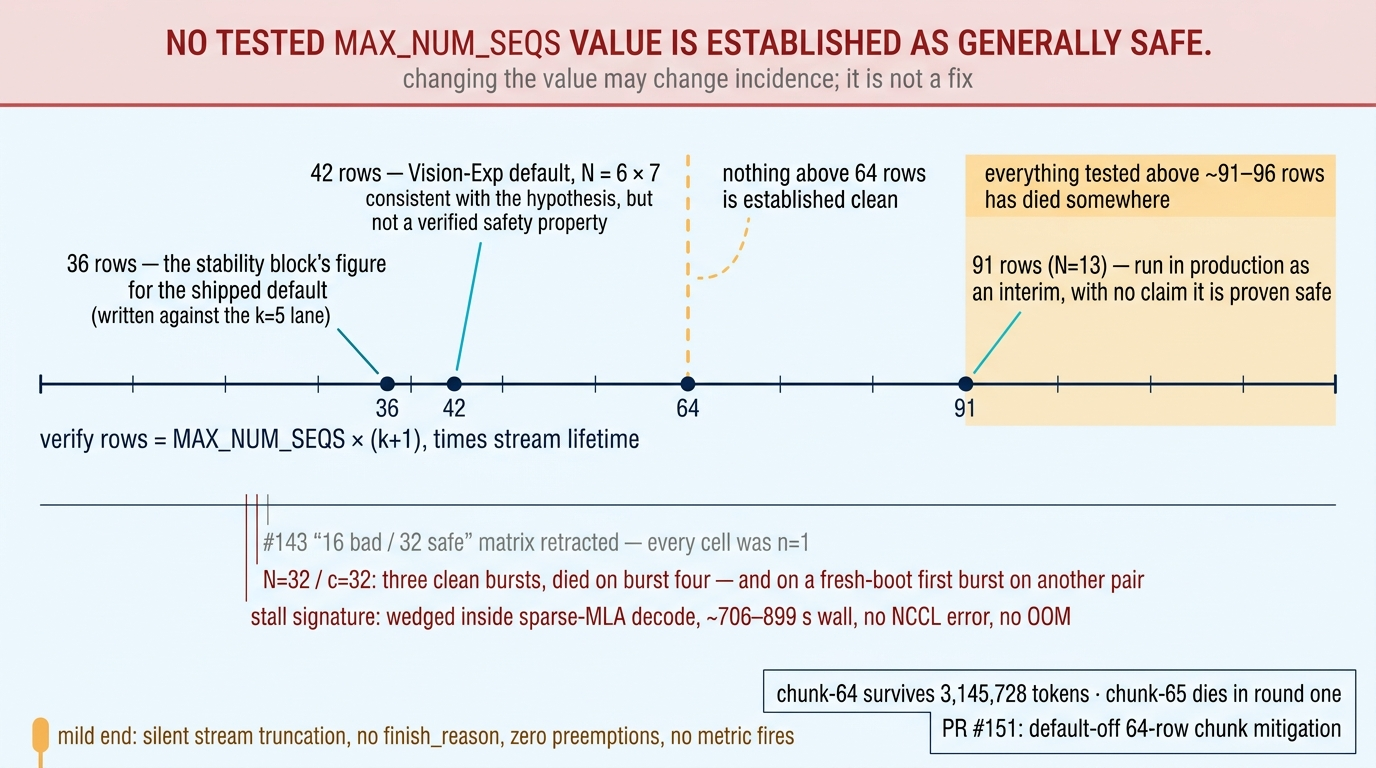
\includegraphics[width=\textwidth]{figures/ch04-verify-rows-141.png}
\caption{The \ghissue{141} evidence on one axis. The best current hypothesis
is geometric --- failure probability rising with verify rows
(\code{MAX_NUM_SEQS} $\times\,(k{+}1)$) times stream lifetime --- but the
evidence is deliberately thin: a retracted $n{=}1$ matrix, stochastic
per-burst stalls, and a production interim its own reporter declines to call
safe. The dashed boundary marks what is not established clean, not a safe
region.}
\label{fig:profile-verifyrows}
\end{figure}

The mild end of the severity spectrum is the dangerous one, because it is
invisible: a short stall cancels the batch, and the result is \emph{silent
stream truncation with no \code{finish_reason}} --- zero preemptions, no
metric fires. \Cref{ch:bugs} follows the full investigation.

\begin{hbwarning}
Two operational rules survive the retraction. No tested
\envvar{MAX_NUM_SEQS} value is established as generally safe under
\ghissue{141}. And if you raise admission, watch for missing
\code{finish_reason} --- it is the earliest signal, well before a watchdog
kill.
\end{hbwarning}

Whatever the profile, concurrent heavy \emph{prefills} remain
scheduler-bound (issues \ghissue{80}/\ghissue{140}): admission tuning raises
decode throughput; it does not fix TTFT contention when several large cold
prompts arrive together.

\section{API authentication}
\label{sec:profile-auth}

Even authentication encodes an incident: the redaction hotfix below is
mandatory and fail-closed because upstream printed keys verbatim. Auth is
optional and enforced by vLLM itself, not a proxy, through two
mutually exclusive variables. \envvar{VLLM_API_KEY} is vLLM's native
single-key env: one bearer key, empty by default (no auth).
\envvar{DSPARK_API_KEYS} is the multi-key form: a single-line,
space/tab-separated list flattened into \emph{one} \code{--api-key} flag ---
the flag is an \code{nargs} list, so repeating it would overwrite rather than
append --- giving each caller an independently revocable key.

If both variables are meaningful, the entrypoint \emph{and} the
start/smoke/status scripts exit 2 naming both, so neither the server nor a
probe ever silently guesses which one applies. Parsing is strict: CR/LF/VT/FF,
backslashes, and any token beginning with \code{-} (which argparse would take
for a vLLM flag) are all rejected with exit 2. The value must live in
\repofile{.env.dspark} --- the launcher sources the file, so an unquoted list
would execute the second key as a command.

Three caveats bound what this auth buys. First, scope: only the prefixes
\code{/v1}, \code{/v2}, and \code{/inference} are guarded. On the pinned
runtime, \code{POST /invocations} and \code{POST /generative_scoring}
\emph{run inference unauthenticated}, and \code{/tokenize},
\code{/detokenize}, \code{/health}, \code{/metrics}, \code{/version}, and
\code{/ping} are likewise keyless --- a keyed deployment still needs
network-level access control on the port (\Cref{fig:profile-apisurface}).

Second, exposure: keys are container argv and environment by design,
readable via host \code{ps} and \code{docker inspect}. Rotation means
editing the line and a full stop/start (no hot reload), and vLLM does not
attribute requests to a key --- this is revocation and blast-radius
control, not per-user logging.

Third, the log channel: upstream's \code{log_non_default_args()} prints
every \code{--api-key} value verbatim at startup. Whenever either variable
is set, the entrypoint therefore requires
\repofile{patches/hotfix-vllm-redact-api-key-log.sh} to apply and verify
(\code{--status}), and fails the container before \code{exec vllm} on any
error --- with no \envvar{DSPARK_SKIP_HOTFIX} bypass. The startup log then
shows \code{'api_key': ['<redacted:N value(s)>']}, preserving the count but
not the bytes.

\begin{figure}[htbp]
\centering
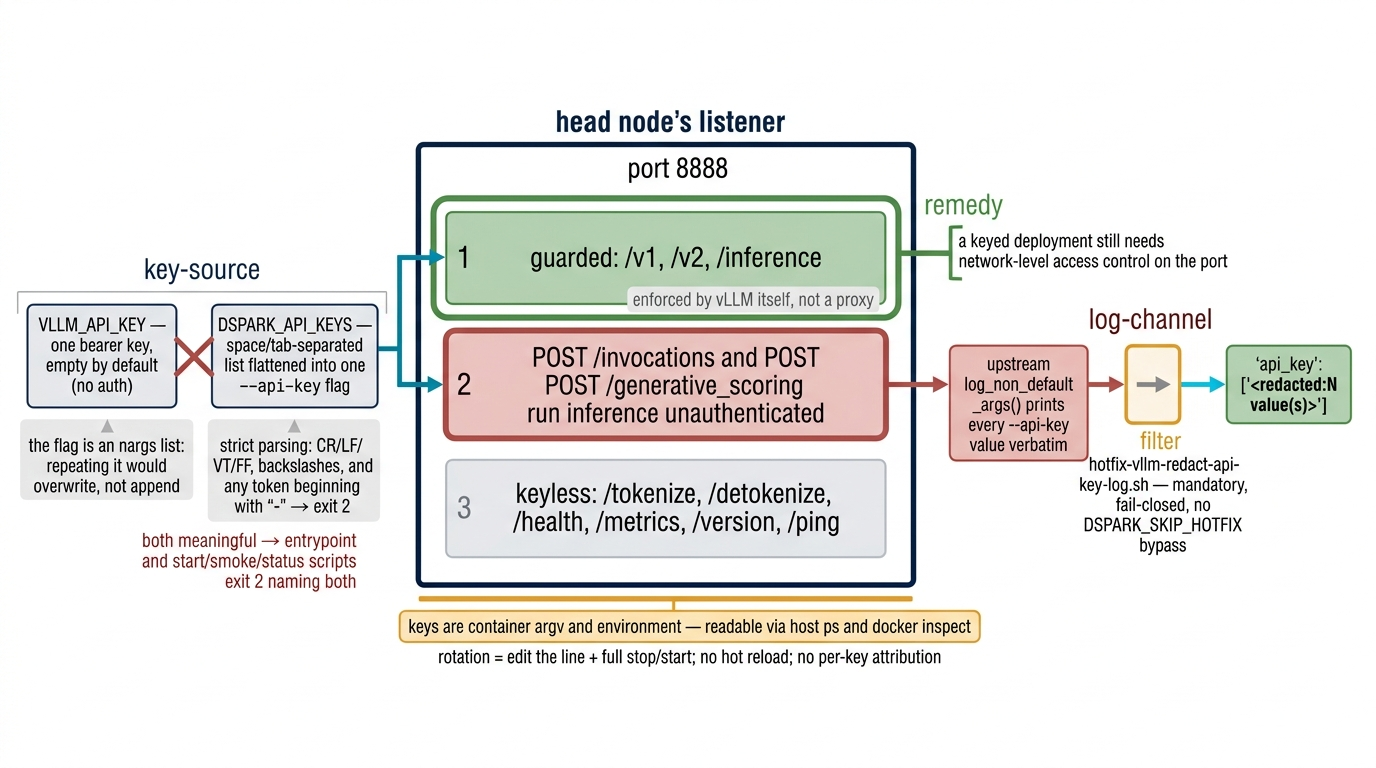
\includegraphics[width=\textwidth]{figures/ch04-api-surface.png}
\caption{What a key buys, and what it does not. vLLM enforces the key on the
\code{/v1}, \code{/v2} and \code{/inference} prefixes only --- two
\code{POST} routes still run inference unauthenticated and six more are
keyless, so network-level access control on the port remains mandatory. The
redaction hotfix is fail-closed with no bypass because upstream prints every
key verbatim at startup.}
\label{fig:profile-apisurface}
\end{figure}

\FloatBarrier
A serving profile stops reading like a list of preferences here. Almost
every value in this argv is either derived from another --- the capture size
from the sequence count and $k$, the utilization from
\envvar{GPU_MEMORY_UTILIZATION_TEXT}, the model from \envvar{ABLITERATED}
--- or the residue of a numbered incident, which is why hand-editing one of
them is how two ranks stop agreeing. And the failures these defaults hold
back are uniformly the quiet kind: a
decode step that silently runs eager, a GID nobody wanted, an answer that
returns null because reasoning spent the budget, a stream that simply stops
with no \code{finish_reason} at all. The flags are the incident log, written
in the only place the engine reads.

\section*{Takeaways}

\begin{itemize}
  \item The serve command is generated, validated, and normalized in stages
    (\repofile{.env.dspark} $\rightarrow$ launcher $\rightarrow$ compose
    $\rightarrow$ entrypoint $\rightarrow$ argv); change knobs at the top and
    never hand-set derived values. \envvar{GPU_MEMORY_UTILIZATION} set by
    hand desynchronizes the ranks, and the CUDA-graph capture size passed
    unrounded --- the arithmetically correct 42 rather than the padded 48
    --- dropped the c=6 step to fully eager at a measured 12\,\% cost
    (122 versus 139~\tokspersec{}). Verify the boot log, not the intention.
  \item Capacity flags are admission ceilings, not reservations: one shared
    pool of 2{,}331{,}430 tokens (17.04\,GiB) is the only thing actually
    spent, the \code{2.22x} boot line answers only the full-1M question, and
    the pool is sized from the minimum across ranks.
  \item \code{max_tokens} counts think plus answer;
    \code{thinking_token_budget} is the precise tool and is doubly opt-in
    (boot flag \ghissue{31} + per-request field), with \ghissue{66} noting a
    decode-cliff risk for omit-field traffic.
  \item To NCCL, defined-empty is not absent: the entrypoint unsets empty
    passthrough keys so config files and per-HCA GID selection are never
    masked --- and on this image a Stage-C-only key is a warn-and-ignore
    no-op, so an unknown-env warning proves nothing either way.
  \item Two things a tuned profile does not buy. Raised admission delivers
    real aggregate throughput (325 \tokspersec{} at c=32), yet no tested
    \code{MAX_NUM_SEQS} is established as generally safe under
    \ghissue{141} --- watch for missing \code{finish_reason}. And an API key
    guards only \code{/v1}, \code{/v2}, and \code{/inference}: two inference
    routes stay open, so network-level access control remains mandatory, as
    does the fail-closed log-redaction hotfix whenever auth is on.
\end{itemize}

\chaptertransition{One rule in this chapter already pointed below the
configuration file. The entrypoint unsets \envvar{NCCL_IB_GID_INDEX}
precisely so that something further down --- NCCL, per HCA --- can make a
choice the profile is not qualified to make, and every number in the profile
assumes that choice comes out right, because both ranks only render the same
argv if the wire between them behaves. That wire carries roughly 108
collectives per decode step and hundreds of megabytes per prefill chunk, and
its arithmetic is uncomfortable the moment you look: each machine advertises
a 200\,Gb QSFP port, and no single PCIe function behind that port can carry
it.}
